\documentclass[11pt]{article}
\usepackage{geometry,marginnote} % Pour passer au format A4
\geometry{hmargin=1cm, vmargin=1cm} % 

% Page et encodage
\usepackage[T1]{fontenc} % Use 8-bit encoding that has 256 glyphs
\usepackage[english,french]{babel} % Français et anglais
\usepackage[utf8]{inputenc} 

\usepackage{lmodern,numprint}
\setlength\parindent{0pt}

% Graphiques
\usepackage{graphicx,float,grffile,units}
\usepackage{tikz,pst-eucl,pst-plot,pstricks,pst-node,pstricks-add,pst-fun,pgfplots} 

% Maths et divers
\usepackage{amsmath,amsfonts,amssymb,amsthm,verbatim}
\usepackage{multicol,enumitem,url,eurosym,gensymb,tabularx}

\DeclareUnicodeCharacter{20AC}{\euro}



% Sections
\usepackage{sectsty} % Allows customizing section commands
\allsectionsfont{\centering \normalfont\scshape}

% Tête et pied de page
\usepackage{fancyhdr} \pagestyle{fancyplain} \fancyhead{} \fancyfoot{}

\renewcommand{\headrulewidth}{0pt} % Remove header underlines
\renewcommand{\footrulewidth}{0pt} % Remove footer underlines

\newcommand{\horrule}[1]{\rule{\linewidth}{#1}} % Create horizontal rule command with 1 argument of height

\newcommand{\Pointilles}[1][3]{%
  \multido{}{#1}{\makebox[\linewidth]{\dotfill}\\[\parskip]
}}

\newtheorem{Definition}{Définition}

\usepackage{siunitx}
\sisetup{
    detect-all,
    output-decimal-marker={,},
    group-minimum-digits = 3,
    group-separator={~},
    number-unit-separator={~},
    inter-unit-product={~}
}

\setlength{\columnseprule}{1pt}

\begin{document}

\horrule{2px}
\section*{Chapitre 1 - Calculer - \texttt{(T)}}
\horrule{2px}

\section*{L'écriture des nombres}

On écrit son cours pour se souvenir et pour être lu. Il faut donc faire un effort d'écriture sur les chiffres et les symboles. On essayera autant que possible d'écrire correctement les grands nombres. 

\begin{itemize}
  \item 0 1 2 3 4 5 6 7 8 9
  \item \nombre{10000}
\end{itemize} 


\section*{L'écriture des calculs}

\begin{itemize}
  \item Les calculs ne s'écrivent pas les uns à la suite des autres. 
  \item On saute une ligne à chaque étape de calcul et on aligne les signes =.
  \item On peut faire plusieurs étapes par ligne. (si on est bon !)
  \item On souligne le résultat.
\end{itemize}

\section*{Les priorités de calcul}

\begin{itemize}
  \item On doit lire le calcul en entier de gauche à droite et le relire à chaque étape.
  \item On commence par les parenthèses.
  \item On fait ensuite les produits et les divisions en lisant de gauche à droite.
  \item On finit par les additions et les soustractions en lisant de gauche à droite.
\end{itemize}


\begin{align*}
  A &= 3 \times (4 + 4) \div 2 - 8 + 13 \\
  A &= 3 \times 8 \div 2 - 8 + 13\\
  A &= 24 \div 2 - 8 + 13 \\
  A &= 12 - 8  + 13\\
  A &= 17 \\
\end{align*}


\textbf{Remarque} : \\
\textit{Attention sur la calculatrice également il est important de bien taper son calcul. } : $8 \div 2(2+2) =$ 16 (TI) ou 1 (Casio)

\begin{figure}[H]
      \centering
      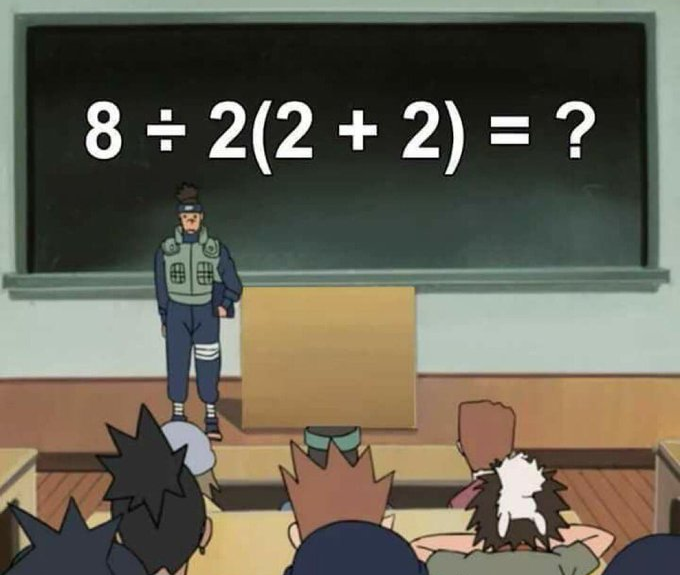
\includegraphics[width=0.4\linewidth]{5x1-calculer/naruto.png}
\end{figure}


\newpage
%impresssion

\textbf{Remarque} : \\
\textit{Attention sur la calculatrice également il est important de bien taper son calcul. } : $8 \div 2(2+2) =$ 16 (TI) ou 1 (Casio)


  \begin{figure}[H]
        \centering
        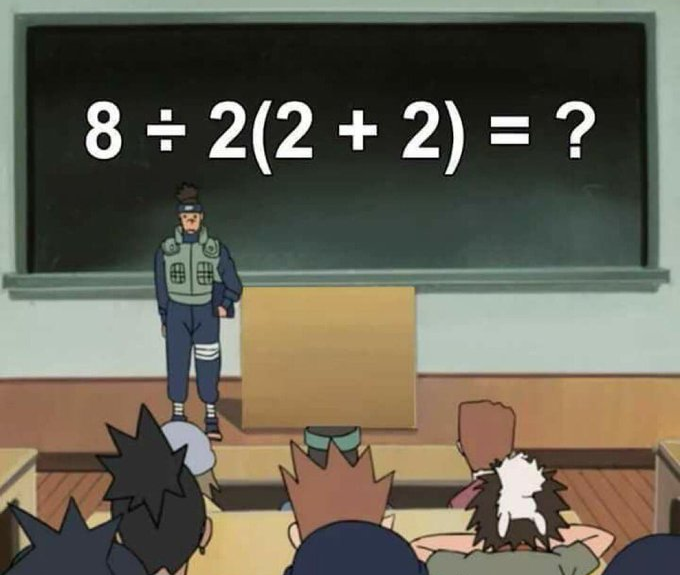
\includegraphics[width=0.4\linewidth]{5x1-calculer/naruto.png}
  \end{figure}




\textbf{Remarque} : \\
\textit{Attention sur la calculatrice également il est important de bien taper son calcul. } : $8 \div 2(2+2) =$ 16 (TI) ou 1 (Casio)

\begin{figure}[H]
      \centering
      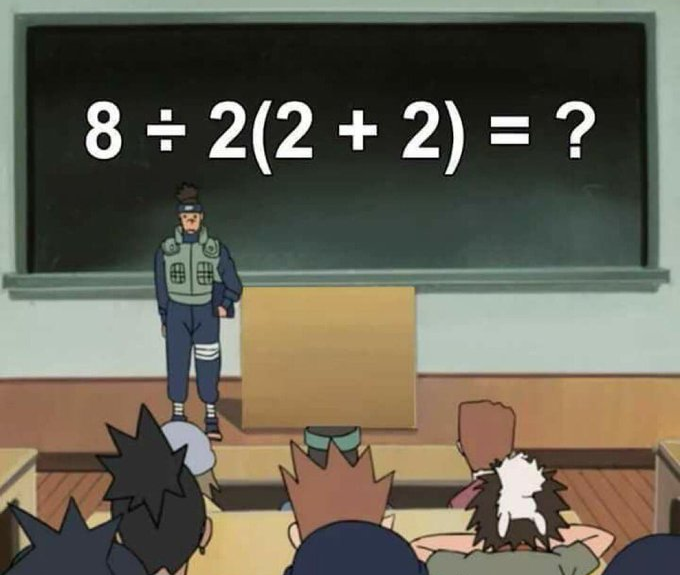
\includegraphics[width=0.4\linewidth]{5x1-calculer/naruto.png}
\end{figure}




\textbf{Remarque} : \\
\textit{Attention sur la calculatrice également il est important de bien taper son calcul. } : $8 \div 2(2+2) =$ 16 (TI) ou 1 (Casio)

\begin{figure}[H]
      \centering
      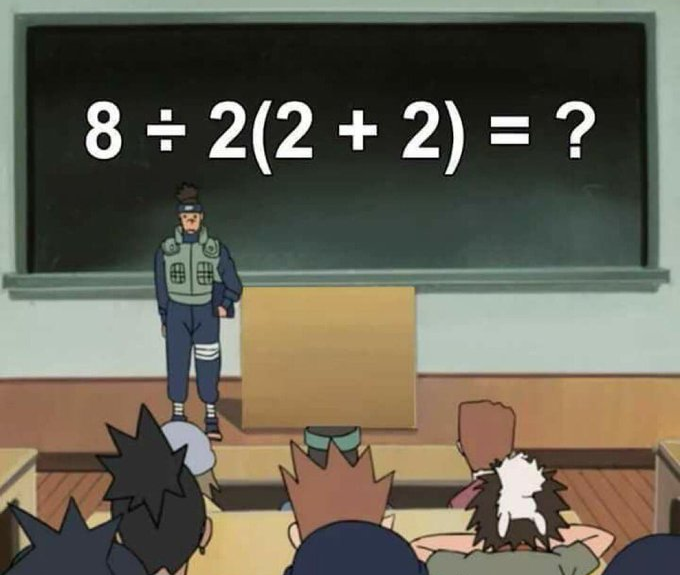
\includegraphics[width=0.4\linewidth]{5x1-calculer/naruto.png}
\end{figure}


\end{document}
